\section{Beispiel 3}

Für einen PNP-Transistor und einen p-Kanal MOSFET sollten bei unterschiedlichen Temperaturen die Übertragungs- und Ausgangskennlinienscharen simuliert werden. Abbildungen \ref{fig:3_pnp_transfer} und \ref{fig:3_pnp_output} zeigen die Übertragungs- und Ausgangskennlinie für einen PNP-Transistor vom Typ Q2N3906, Abbildungen \ref{fig:3_pmos_transfer} und \ref{fig:3_pmos_output} zeigen die Übertragungs- und Ausgangskennlinie für einen p-Kanal MOSFET vom Typ IRF9140. Dabei wurden die Simulationen für mehrere $V_{CE}$ bzw. $V_{DS}$ mit Hilfe eines \emph{Nested Sweep} durchgeführt (es wurden nicht zu viele Werte gewählt, sodass das Diagramm übersichtlich bleibt). Weiters wurden die Simulationen bei unterschiedlichen Temperaturen durchgeführt. Die Kurven sind beschriftet und haben in allen Diagrammen die gleiche Farbgebung (grün...-10°C, rot...27°C, blau...85°C). Man kann die Temperaturabhängigkeit von $V_{BE}$ des PNP-Transistors gut erkennen.

\begin{figure}[h!]
	\centering
	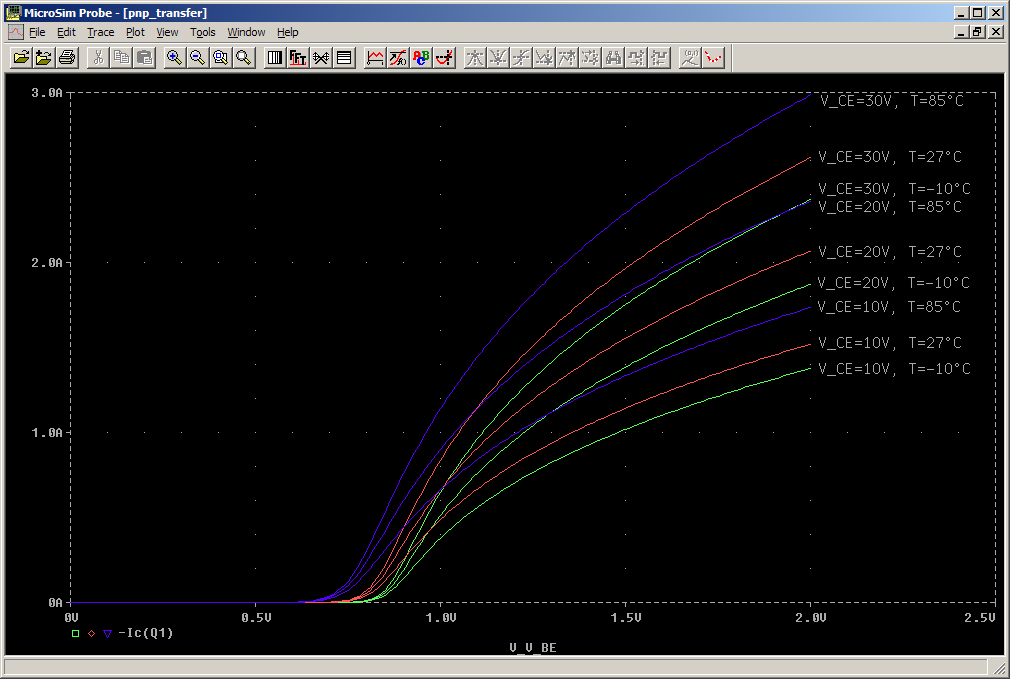
\includegraphics[width=0.70\textwidth]{fig/ue2_ex3_pnp_transfer.PNG}
	\caption{Übertragungskennlinie des Q2N3906}
	\label{fig:3_pnp_transfer}
\end{figure}

\begin{figure}[h!]
	\centering
	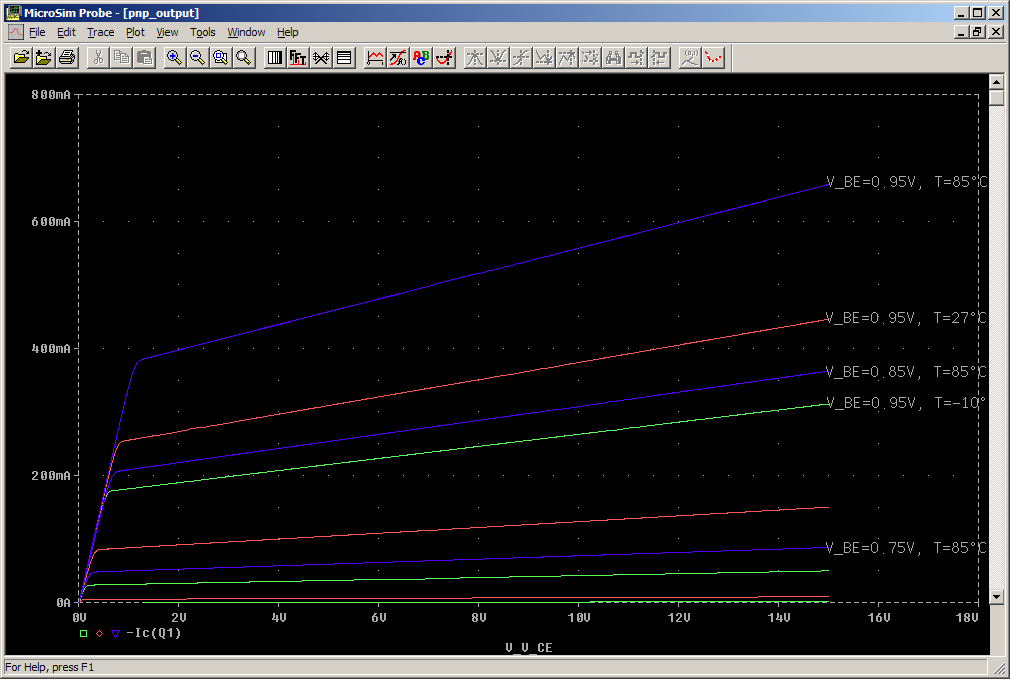
\includegraphics[width=0.70\textwidth]{fig/ue2_ex3_pnp_output.PNG}
	\caption{Ausgangskennlinie des Q2N3906}
	\label{fig:3_pnp_output}
\end{figure}

\begin{figure}[h!]
	\centering
	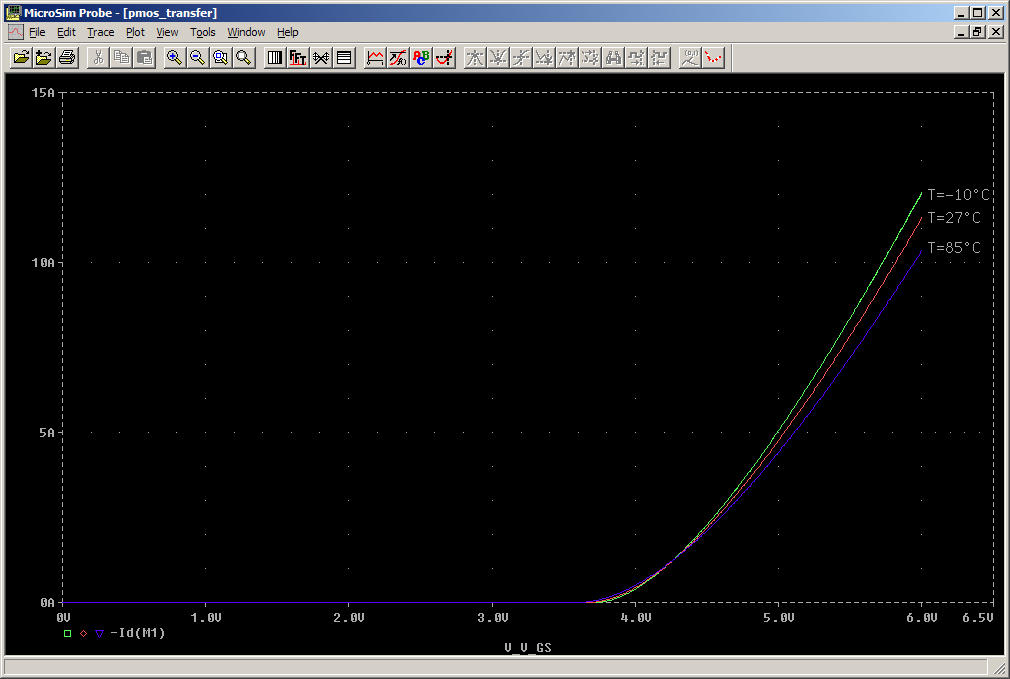
\includegraphics[width=0.70\textwidth]{fig/ue2_ex3_pmos_transfer.PNG}
	\caption{Übertragungskennlinie des IRF9140}
	\label{fig:3_pmos_transfer}
\end{figure}

\begin{figure}[h!]
	\centering
	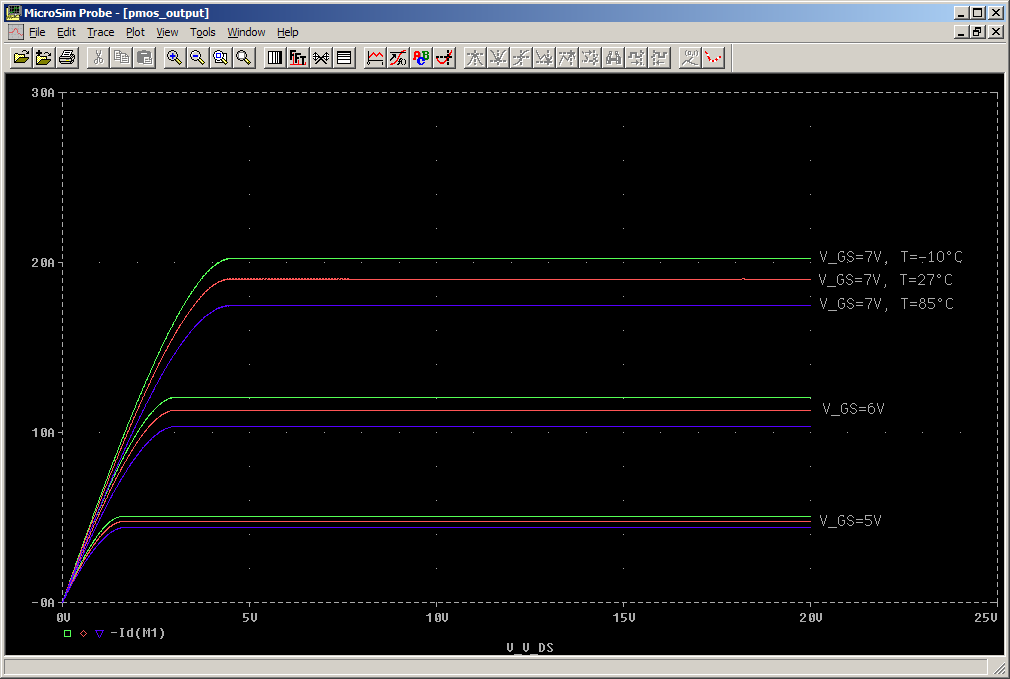
\includegraphics[width=0.70\textwidth]{fig/ue2_ex3_pmos_output.PNG}
	\caption{Ausgangskennlinie des IRF9140}
	\label{fig:3_pmos_output}
\end{figure}


Abbildungen \ref{fig:3_pnp_s} und \ref{fig:3_pnp_s_norm} zeigen die Steilheit des PNP-Transistors $S = \frac{dI_C}{dV_{BE}}$ und die auf den Strom normierte Steilheit $S_{norm} = \frac{S}{I_C}$. Die maximalen Steilheiten werden im Bereich von $V_{BE}$ erreicht, bei dem der Transistor zu leiten beginnt.

\begin{figure}[h!]
	\centering
	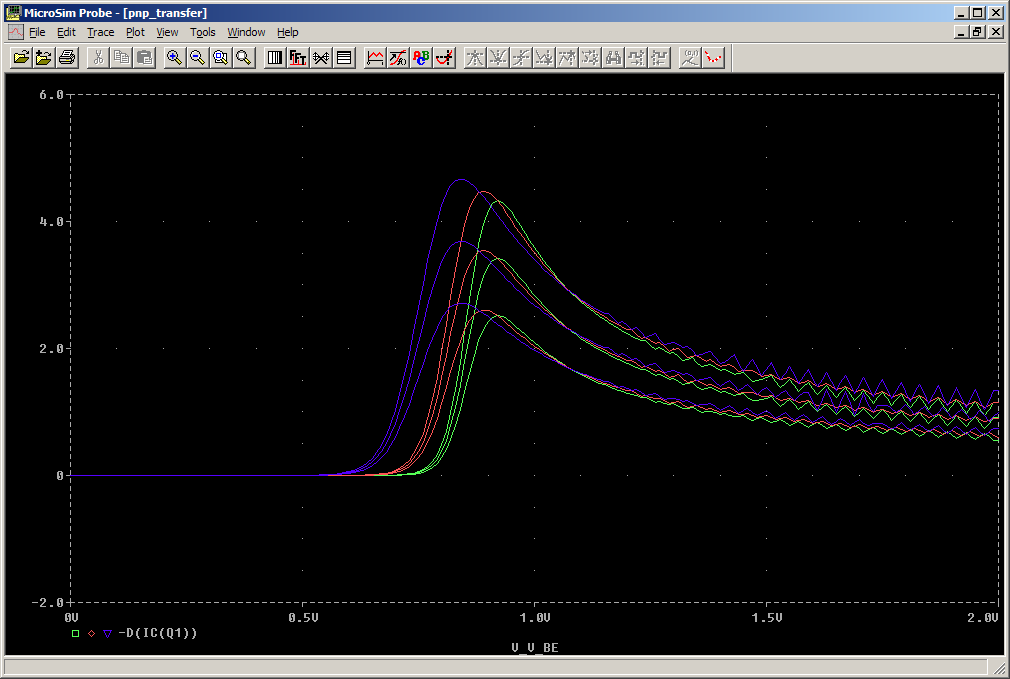
\includegraphics[width=0.70\textwidth]{fig/ue2_ex3_pnp_s.PNG}
	\caption{Steilheit des Q2N3906}
	\label{fig:3_pnp_s}
\end{figure}

\begin{figure}[h!]
	\centering
	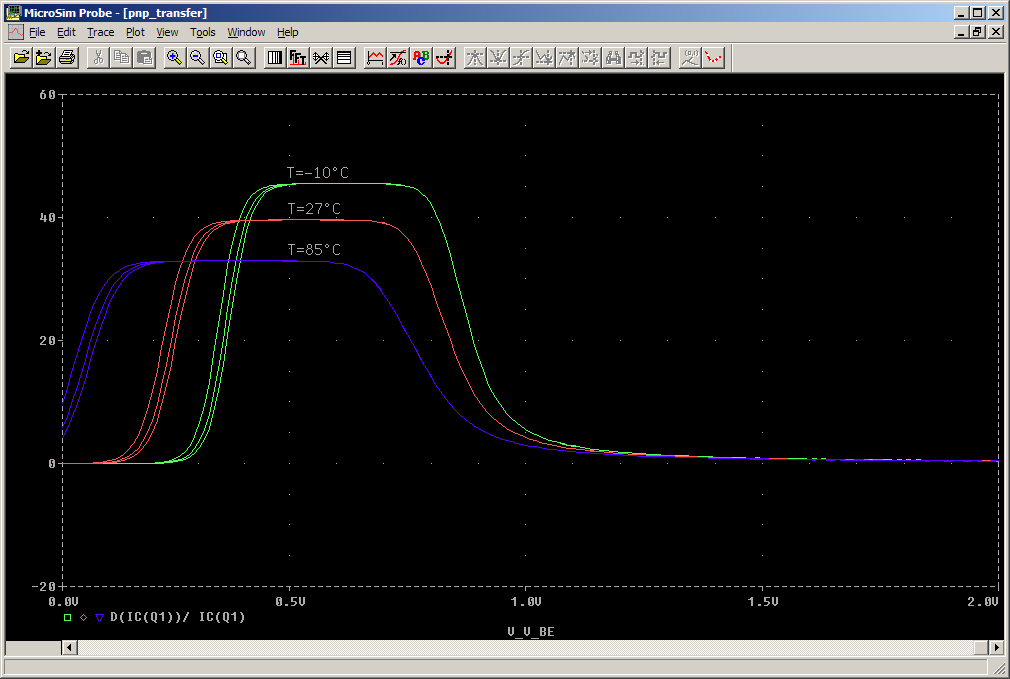
\includegraphics[width=0.70\textwidth]{fig/ue2_ex3_pnp_s_norm.PNG}
	\caption{Normierte Steilheit des Q2N3906}
	\label{fig:3_pnp_s_norm}
\end{figure}

Abbildungen \ref{fig:3_pmos_s} und \ref{fig:3_pmos_s_norm} zeigen die Steilheit des p-Kanal MOSFET $g_m = \frac{dI_D}{dV_{GS}}$ und die auf den Strom normierte Steilheit $g_m_{norm} = \frac{g_m}{I_D}$. Man erkennt, dass die maximale Steilheit nur in einem sehr schmalen Bereich verfügbar ist.

\begin{figure}[h!]
	\centering
	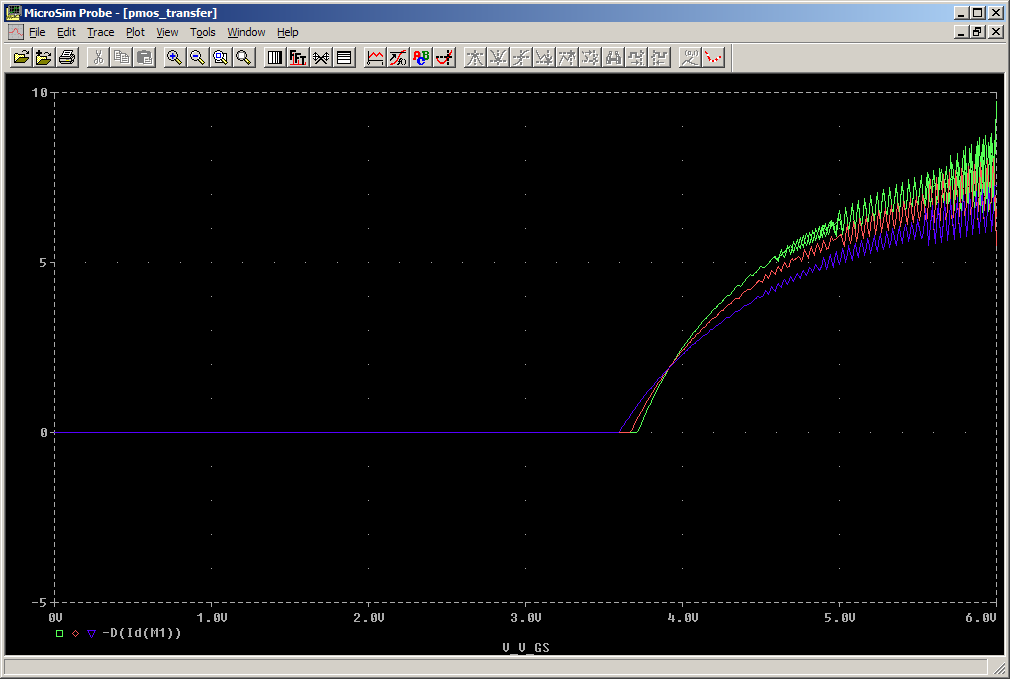
\includegraphics[width=0.70\textwidth]{fig/ue2_ex3_pmos_s.PNG}
	\caption{Steilheit des IRF9140}
	\label{fig:3_pmos_s}
\end{figure}

\begin{figure}[h!]
	\centering
	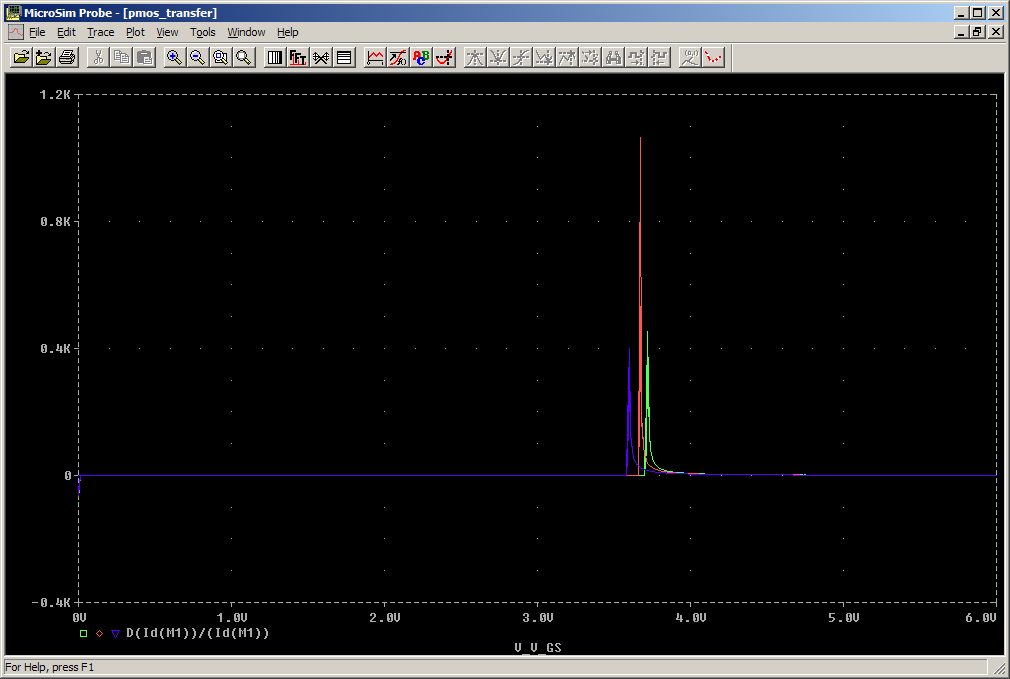
\includegraphics[width=0.70\textwidth]{fig/ue2_ex3_pmos_s_norm.PNG}
	\caption{Normierte Steilheit des IRF9140}
	\label{fig:3_pmos_s_norm}
\end{figure}

